% 30/12/2015 06:22 %

\section{M-SPLear\allowbreak ning Experimental Evaluation}\label{section3}

%In this section, an experimental evaluation of M-SPLear\allowbreak ning regarding time-to-market and quality improvement in generating mobile learning applications is reported. M-SPLear\allowbreak ning was compared with a singular software development methodology. This study, we called as singular methodology the process of software development in which developers use only their own knowledge to develop mobile learning applications from scratch, without any reuse or support technique.  

In this section, an experimental evaluation of M-SPLear\allowbreak ning regarding time-to-market and quality improvement in generating mobile learning applications is reported. M-SPLear\allowbreak ning was compared with a singular software development methodology. It was adopted the term singular methodology as the process of software development in which developers use only their own knowledge to develop mobile learning applications from scratch, without any reuse or support technique.  

The guidelines proposed by Wohlin et al \cite{wohlin12} and the report template suggested by Jedlitschka and Pfahl \cite{jedlitschka07} were followed for the conduction of this controlled experiments.

\subsection{Motivation}\label{sub:motivation}


The choice for the adoption of new technologies or approaches used in the development process depends on several aspects of quality. Although many approaches have been developed, many issues about them must be solved for a suitable adoption in both industry and academic environments. Experimental evaluations may shed light on the identification of evidence from quality and benefits of an approach, justifying its choice. In some cases, the collected evidence may still support the correction of problems identified during the experimental evaluations and improvements in the proposals \cite{wohlin12,juristo10}.

Therefore, the experimental evaluation of M-SPLear\allowbreak ning is presented based on two relevant software development variables: time-to-market and number of faults. These variables can be directly influenced by the adopted development methodology and approaches that support the variabilities and commonalities management \cite{hubaux10,capilla13}. Additionally, in industry, quality and time-to-market, such as other variables, can define the success or unsuccess of the business to satisfactorily attend their clients \cite{hubaux10}. Thus, we select these variables to be experimentally compared in our study, considering the influence in the adoption of a concise variability management approach in the design phase of the M-SPLear\allowbreak ning.


\subsubsection{Research Objective}\label{sub:object}

The experiment aimed at \textbf{comparing} a singular software development (SSD) and the software product line (SPL) methodologies, \textbf{for the purpose of} identifying the most efficient, \textbf{with respect to} the time spent on the creation of software products and the number of faults found, from the point of view of software engineers \textbf{in the context of} practitioners from industry.


\subsection{Experimental Design}\label{sub:design}

This section describes the experimental design and procedures for support of future replications. In this sense, all the planning, configuration of environment, dynamics of execution and tests are in the experimental package, available on the project website\footnote{\url{http://falvojr-msc.github.io/msplearning}}.

\subsubsection{Goals}

Two research questions (R.Q.) based on the research objective were raised:

\begin{itemize}
\setlength\itemsep{0.8em}
\item \textbf{R.Q.1} Which methodology is more efficient regarding time-to-market -- singular software development (SSD) or SPL software product line (SPL)?
\item \textbf{R.Q.2} Which methodology presents more quality, in terms of number of faults, in the software product created -- SSD or SPL?
\end{itemize}

\subsubsection{Hypotheses}

Two sets of hypotheses were defined to be tested and each of them is related to its respective research questions (R.Q.1 and R.Q.2):

\vspace{1em}
\textbf{R.Q.1 hypotheses:} time-to-market

	\begin{itemize}
    \setlength\itemsep{0.8em}
	\item \textbf{Null Hypothesis ($H_{0}$)}: there is no significant difference of time-to-market between SSD and SPL. $(H_{0}$ : $\mu$(\textit{t(SSD)}) =  $\mu$(\textit{t(SPL)}));
	
	\item \textbf{Alternative Hypothesis ($H_{1}$)}: SSD has less time-to-market than SPL. 	($H_{1}$ : $\mu$(\textit{t(SSD)}) $<$ $\mu$(\textit{t(SPL)}));
		
	\item \textbf{Alternative Hypothesis ($H_{2}$)}: SSD has more time-to-market than SPL. 	($H_{2}$ :  $\mu$(\textit{t(SSD)}) $>$ $\mu$(\textit{t(SPL)})).		
	\end{itemize}	

\vspace{1em}
\textbf{R.Q.2 hypotheses:}
quality, in terms of number of faults
	\begin{itemize}
    \setlength\itemsep{0.8em}
	
	\item \textbf{Null Hypothesis ($H_{0}$)}: there is no significant difference between SSD and SPL with regard to quality regarding the number of faults in the software products created. 	($H_{0}$ : $\mu$(\textit{d(SSD)}) =  $\mu$(\textit{d(SPL)}));
	
	\item \textbf{Alternative Hypothesis ($H_{1}$)}: SSD has a larger number of faults than SPL. ($H_{1}$ : $\mu$(\textit{d(SSD)}) $>$ $\mu$(\textit{d(SPL)}));
		
	\item \textbf{Alternative Hypothesis ($H_{2}$)}: SSD has a smaller number of faults than SPL. ($H_{2}$ :  $\mu$(\textit{d(SSD)}) $<$ $\mu$(\textit{d(SPL)})).		
	
	\end{itemize}

\subsubsection{Variables}

Dependent variables are time ($t$) and faults ($f$), defined as follows:

\small

\begin{equation}\label{eq:1}
\mu{(t)}=(\Sigma xi)/n, i = 1..n
\end{equation}
\begin{equation}\label{eq:2}
\mu{(f)}=(\Sigma yi)/n, i = 1..n
\end{equation}
\normalsize 

where:

- \textit{t} is the implementation time (minutes);

- \textit{f} is the number of faults;

- \textit{xi} is the time of implementation of participant i;

- \textit{yi} is the number of faults detected in the implementation of participant i;

- \textit{n} is the total of participants in the experiment.

\normalsize


\vspace{5mm}


Independent variables are the development methodology, which is a factor with two treatments (SSD and SPL), and the software product configuration for mobile learning platform, which is a factor with two treatments, namely product 1 (P1) and product 2 (P2). Table \ref{tab:variables} shows the description of dependent and independent variables.

\begin{table}[ht]
\centering
\caption{Dependent and Independent Variables Description.}
\label{tab:variables}

\resizebox{1.0\textwidth}{!}{%
\begin{tabular}{|c|c|c|c|c|c|c|c|c|c|}
\hline
\textbf{\begin{tabular}[c]{@{}c@{}}Name of \\ the Variable\end{tabular}} & \textbf{\begin{tabular}[c]{@{}c@{}}Type of \\ the Variable\end{tabular}} & \textbf{Abbrev.} & \textbf{Class} & \textbf{Entity} & \textbf{\begin{tabular}[c]{@{}c@{}}Type of \\ Attribute\end{tabular}} & \textbf{\begin{tabular}[c]{@{}c@{}}Scale \\ Type\end{tabular}} & \textbf{Unit} & \textbf{Range} & \textbf{\begin{tabular}[c]{@{}c@{}}Counting \\ Rule\end{tabular}} \\ \hline
\begin{tabular}[c]{@{}c@{}}Development \\ methodology\end{tabular} & Independent & DM & Method & \begin{tabular}[c]{@{}c@{}}Software \\ development \\ methodology\end{tabular} & N/A & Nominal & N/A & SSD and SPL & N/A \\ \hline
\begin{tabular}[c]{@{}c@{}}Software \\ products\end{tabular} & Independent & P & Product & \begin{tabular}[c]{@{}c@{}c@{}}Mobile \\ software \\ product\end{tabular} & N/A & Nominal & N/A & P1 and P2 & N/A \\ \hline
\begin{tabular}[c]{@{}c@{}}Time of \\ implementation\end{tabular} & Dependent & t(3) & Product & \begin{tabular}[c]{@{}c@{}}Time to \\ market\end{tabular}  & \begin{tabular}[c]{@{}c@{}}Internal: time; \\ external: time \\ to market.\end{tabular} & Ordinal & Minutes & \begin{tabular}[c]{@{}c@{}}From 00:00:00 \\ to 03:00:00\end{tabular} & Eq. 1 \\ \hline
Faults & Dependent & f(4) & Product & \begin{tabular}[c]{@{}c@{}c@{}c@{}}Number of \\ faults \\ in each \\ software \\ product\end{tabular} & \begin{tabular}[c]{@{}c@{}}Internal: faults; \\ external: quality.\end{tabular} & Ordinal & Integer & Any integer & Eq. 2 \\ \hline
\end{tabular}%
}
\end{table}

Time-to-market is the time spent, in average, for the implementation of a software product with a specific group of variabilities of M-SPLear\allowbreak ning. With regard to the number of faults, the implemented products were tested using the concept of test cases \cite{craig02}. Thus, it was possible to quantify the mean of defects of products. Such metrics are relevant since they are directly related to time-to-market and quality of the m-learning applications. Additionally, they are relevant metrics for development industry\cite{JABANGWE201898}.

\subsubsection{Participants}

In our study, the participants were employees (volunteers) from a Brazilian software development industry. All of them had, at least, one year of experience with development background in Java, Microsoft .NET and/or PHP.

The small number of practitioners (18) led us to apply a non-random selection. The random capacity was applied at the assignment of the development methodology and software product by participant. 

It is important to highlight that, even with a small number of participants and a reduced statistical power, this experimental evaluation is important since it allows the collection of initial evidence about the compared methodologies. Besides, the sample can be increased in future replications \cite{falessi2017,host2000}.

Block classification was defined by two factors with two treatments, which were interspersed in four groups. The population was divided into four blocks by means of a draw. The balancing was applied in the tasks, which were assigned in equal numbers to a similar number of participants.

%The 18 participants were randomly separated into the following groups with a total of 9 participants each:

The 18 participants were randomly separated into groups of nine participants each:

\begin{itemize}
\item \textbf{First Group:} focused on SSD with P1 and SPL with P2;

\item \textbf{Second Group:} focused on SPL with P1 and SSD with P2;

\item \textbf{Third Group:} focused on SSD with P2 and SPL with P1; and

\item \textbf{Fourth Group:} focused on SPL with P2 and SSD with P1;
\end{itemize}

\subsubsection{Objects}

Among a total of 30 features and different configurations, two educational software products configurations for mobile learning platform (Android) were considered for the application of the SSD and SPL methodologies, which were: one for image (P1) and one for video resource (P2).

\subsubsection{Instrumentation}

The experiment was supported by the following set of instruments: (i) similar desktop computers with all necessary tools (Eclipse IDE and plugins); (ii) the consent term for the experimental study; (iii) a characterization questionnaire; (iv) use case, component and sequence UML diagrams; (v) interface messages; (vi) database model; (vii) a project base; (viii) similarities of the products; and (ix) experimental forms for SSD and SPL, randomly distributed and feedback questionnaire.

\subsubsection{Data Collection and Analysis Procedures}

The main assessment tools were the products developed based on two software specifications (P1 and P2) for mobile learning platform (Android), also available in the experimental package.

The M-SPLear\allowbreak ning was designed according to the catalog of requirements (Section \ref{section2}) and with 30 features, 16 mandatory and 14 optional for m-learning applications. A specific niche of features was used for the evaluation. The variabilities related to multimedia resources enabled the creation of up to 15 different products. P1 and P2 were specified and implemented by SSD and SPL methodologies. Figure \ref{fig:prod} shows the nuances between the products generated for the video feature.

%REMOVI (linha 157 - não achei a figura de referência):  (represented in Figure \ref{figureMSPLFeatureModel}) 

\begin{figure*}[!ht]
\centering
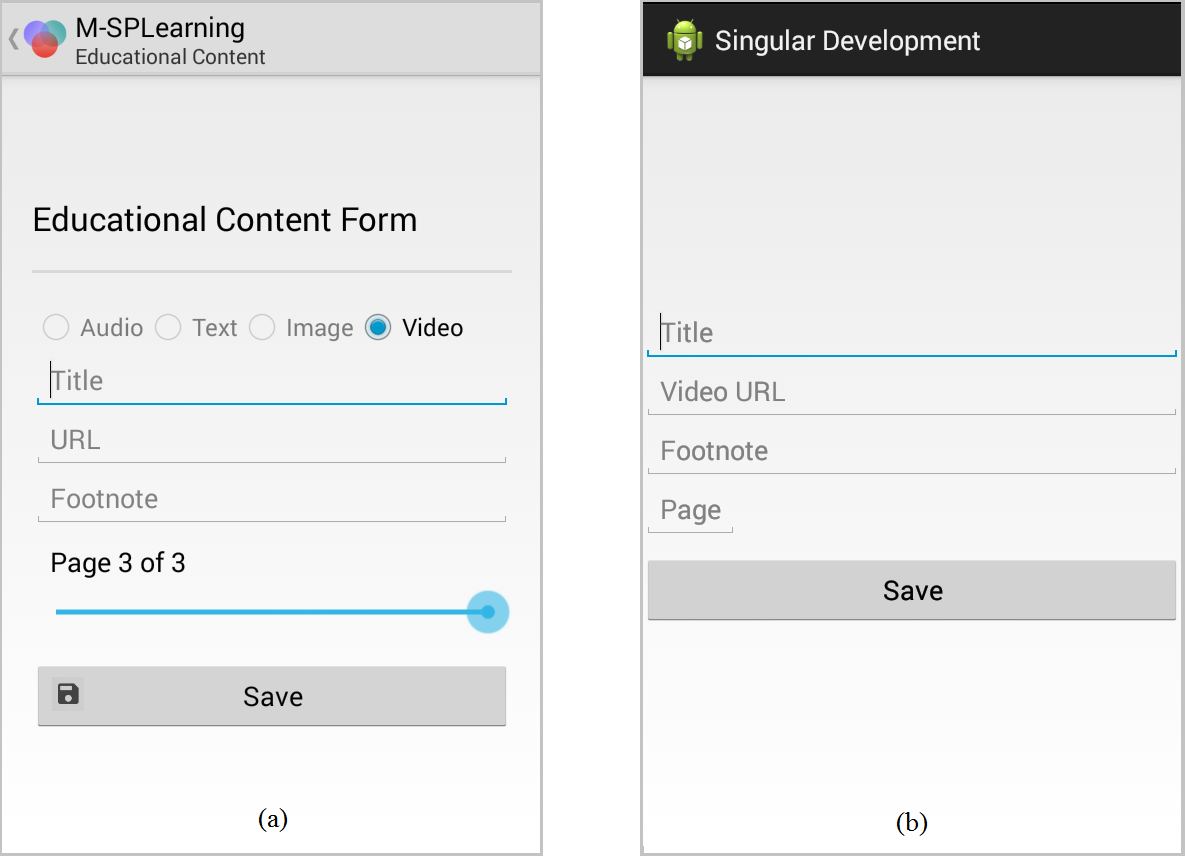
\includegraphics[width=0.69\textwidth]{MSPLGeneratedProducts.png}
\centering
\caption{Two Video Products (P1) Developed in the Experimental Execution with: (a) SPL and (b) SSD.}
\label{fig:prod}
\end{figure*}


To collect the data for the analysis of time-to-market, the initial and final time of implementation process for P1 and P2, was registered individually in the experimental form to be calculated in Equation \ref{eq:1}. On the other hand, for the analysis of quality, each of 15 developed products were tested and the number of faults was collect to compare the use of SPL and SSD methodologies by means of the Equation \ref{eq:2}.

\subsubsection{Validity Evaluation}

A pilot project was developed with two practitioners from industry, who evaluated the study instrumentation and established the duration of the training and execution sessions. The results and these participants were not considered in the final execution and data analysis of the experiment.

\subsection{Execution}\label{sub:execution}

This section presents how the experimental plan (design) was defined.

\subsubsection{Sample}

The sample was composed of a total of 21 practitioners, who participated in the training session. However, 18 participants contributed in the experimental execution, due the unavailability of three volunteers in the execution day.

\subsubsection{Preparation}

The participants underwent a three-day training session, in which were considered the essential concepts of Android development for SSD and SPL with the Eclipse IDE. The knowledge was evaluated through essays at the end of each training session. On the fourth day, the experiment was performed.

\subsubsection{Data Collection}

The steps adopted for data collection were:

\begin{enumerate}

\item The participants attended three days (four hours each day) of training sessions in an industrial environment;

\item The participants were divided into four groups by means of a draw;

\item The experimenter gave participants a set of documents containing UML diagrams, a dataset model and an interface message specification for each product, such as the material used in training session. Each participant was provided with a desktop computer with all requirements to develop a software product and an experimental form to register the spent time with the development process.
\item The participant read each given document;
\item The experimenter explained the documents;
\item The participant read and clarified possible doubts about the products specifications;
\item Each participant received and used two randomly drawn methodologies for the development of a requested m-learning product. For each application, participants registered the lasting of the application (start time, end and breaks). At the end of the two development tasks, for the two methodologies, they were asked to answer a feedback questionnaire and their opinion about the experimental execution and technologies used.
\end{enumerate}

\subsection{Analysis}\label{sub:analysis}

As the experiment session was finished, collected data was prepared (tabulation and descriptive statistics) in order to apply the statistical tests.

\subsubsection{Collected Data and Descriptive Statistics}

For each participant (``\texttt{Participant \#}'' column), we collected the following data: total time of implementation and total number of faults, identified by testing procedures, and the mean calculation. These results are shown in Table \ref{tab:resul1} and the results for each participant are plotted in box-plots of Figure \ref{fig:boxplot}. 

\begin{table}[ht]
\small
\centering
\caption{SSD and SPL Collected Data and Descriptive Statistics.}
\label{tab:resul1}
\resizebox{0.60\textwidth}{!}{%
\begin{tabular}{|c|c|c|c|c|}
\hline
\textbf{} & \multicolumn{2}{c|}{\textbf{SSD}} & \multicolumn{2}{c|}{\textbf{SPL}} \\ \hline
\textbf{Participant \#} & \textbf{Time (t)} & \textbf{Faults (f)} & \textbf{Time (t)} & \textbf{Faults (t)} \\ \hline
1 & 161 & 15 & 2 & 9 \\ \hline
2 & 90 & 8 & 1 & 0 \\ \hline
3 & 105 & 4 & 11 & 0 \\ \hline
4 & 104 & 1 & 3 & 0 \\ \hline
5 & 73 & 2 & 1 & 0 \\ \hline
6 & 99 & 9 & 3 & 0 \\ \hline
7 & 165 & 12 & 10 & 0 \\ \hline
8 & 95 & 1 & 3 & 0 \\ \hline
9 & 104 & 3 & 2 & 0 \\ \hline
10 & 102 & 0 & 4 & 0 \\ \hline
11 & 61 & 0 & 2 & 0 \\ \hline
12 & 82 & 4 & 8 & 0 \\ \hline
13 & 114 & 1 & 4 & 0 \\ \hline
14 & 103 & 6 & 14 & 0 \\ \hline
15 & 111 & 2 & 2 & 0 \\ \hline
16 & 176 & 9 & 4 & 0 \\ \hline
17 & 120 & 17 & 5 & 0 \\ \hline
18 & 175 & 34 & 2 & 9 \\ \hline
\textbf{Mean} & \textbf{113.33} & \textbf{7.11} & \textbf{4.50} & \textbf{1.00} \\ \hline
\textbf{Median} & \textbf{104} & \textbf{4} & \textbf{3} & \textbf{0} \\ \hline
\textbf{Std. Dev.} & \textbf{33.98} & \textbf{8.46} & \textbf{3.75} & \textbf{2.91} \\ \hline
\end{tabular}%
}
\end{table}

\begin{figure*}[!ht]
\centering
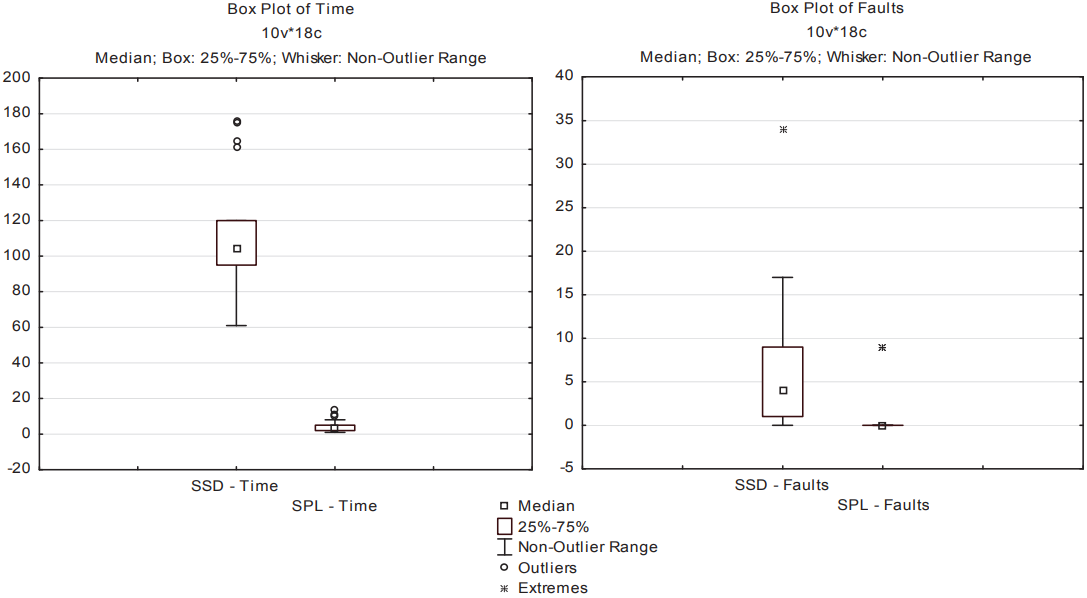
\includegraphics[width=1.0\textwidth]{MSPLBoxplotN.png}
\centering
\caption{Collected Data Box-Plot from SSD/SPL time-to-market and SSD/SPL faults.}
\label{fig:boxplot}
\end{figure*}

\subsubsection{Hypothesis Testing}

Based on the results obtained by the use of SSD and SPL to the development of two mobile learning products, we summarize, analyze and interpret the SSD and SPL collected data (Table \ref{tab:resul1} and Figure \ref{fig:boxplot}) by means of the Shapiro-Wilk normality test and the Mann-Whitney-Wilcoxon hypothesis test. Both tests validated the statistical power of the sample, allowing test the hypotheses.

\subsubsection{Efficiency in the Time of Implementation (R.Q.1)}

\begin{itemize}
\setlength\itemsep{0.8em}

\item \textbf{Collected Data Normality Tests:} Shapiro-Wilk \cite{shaphirowilk65} normality test was applied to SSD and SPL time and faults. The following results were obtained:\\

\textbf{\textit{SSD time (\textit{N}=18):}}

For mean value ($\mu$) of 113.33 and standard deviation value of ($\sigma$) 33.98, the time for the SSD was \textit{p} = 0.0274.

In the \textit{Shapiro-Wilk} test for a sample size \textit{(N)} 18 with 95\% of significance level ($\alpha$ = 0.05), \textit{p} = 0.0274 (0.0274 $<$ 0.05) and calculated value of \textit{W} = 0.8813 $<$ \textit{W} = 0.8970, the sample is considered non-normal.

\textbf{\textit{SPL time (\textit{N}=18):}}

For mean value ($\mu$) of 4.50 and standard deviation value of ($\sigma$) 3.75, the time for the SPL was \textit{p} = 0.0014.

For a sample size \textit{(N)} 18 with 95\% of significance level ($\alpha$ = 0.05), \textit{p} = 0.0014 (0.0014 $<$ 0.05) and calculated value of \textit{W} = 0.7978 $<$ \textit{W} = 0.8970, the sample is considered non-normal.

\item \textbf{Mann-Whitney-Wilcoxon for SSD and SPL time samples:} a rank with weights was assigned to each sample value. The weights were added and applied in Equation \ref{eq:MWW}:
\small
\begin{equation}
\label{eq:MWW}
U(DM) = N_1 * N_2 + \frac{N_1*(N_1+1)}{2} - \sum_{i=1}^{n} total_{2}
\end{equation}
\normalsize 

where:

- \textit{$U(DM)$} is the equation for each independent sample (DM);

- \textit{$N_1$} is the size of the sample for the X methodology;

- \textit{$N_2$} is the size of the sample for the compared methodology (Y);

- \textit{$total_{2}$} is the sum of the weights given for the compared methodology.
\normalsize 
\vspace{5mm}

The time values calculated by Equation \ref{eq:MWW} were 326.5 for SSD and 0.00 for SPL. Each weight matches the participants weights of development process time with SSD or SPL methodology. There is evidence that both values are different ($326.5>0$), which leads to the rejection of the null hypothesis ($H_0$) and acceptance of the alternative hypothesis ($H_{2}$).

Therefore, the answer to R.Q.1 is: SPL is more efficient than the SSD to implement software products for mobile platform taking into account the products P1 and P2 specification. The implementations of the base project and SPL were also considered in the experiment.

The participants received the base project of the two software products to be developed with SSD or SPL. It consisted of similarities of the products and was developed to reduce the experimental execution duration. It was implemented in 480 minutes (8 hours).

Based on the time spent in the development of each software product, it is possible to make some estimates related with the time efforts for both SSD and SPL methodologies evaluated. If considered the time required for the implementation of each base project adopting the SSD methodology, plus the total development time to each participants (480 minutes), the total time would be 10680 minutes or 178 hours ($total_{time}$((subje\allowbreak cts(18) x minutes(480)) + 2040 = 10680 minutes). 

On the other hand, taking into account the base project developing with SPL methodology, the time spent by the 18 participants was 81 minutes (1 hour and 21 minutes) and the total time would be 11361 minutes or 189 hours and 35 minutes ($total_{time}$((participants(18) x minutes(4.5)) + 10599 = 11361 minutes). 

Comparing the values, we notice that the SPL development spent 621 minutes (11 hours and 35 minutes) more than SSD. However, after the SPL implementation, this approach allows the evolution and insertion of new variabilities, assuring the faster generation of new products in addition to other advantages of the adoption of SPL approach.

\end{itemize}

\subsubsection{Number of faults of the created software products (R.Q.2)}

\begin{itemize}
\setlength\itemsep{0.8em}

\item \textbf{Collected Data Normality Tests:} 

\textbf{\textit{SSD faults (\textit{N}=18):}}

For a mean value ($\mu$) 7.11 and standard deviation value of ($\sigma$) 4, the fault for the SSD was \textit{p} = 0.0006 for the \textit{Shapiro-Wilk} normality test.

For a sample size \textit{(N)} 18 with 95\% significance level ($\alpha$ = 0.05), \textit{p} = 0.0006 (0.0006 $<$ 0.05) and value of \textit{W} = 0.7740 $<$ \textit{W} = 0.8970, the sample is considered non-normal.

\textbf{\textit{SPL faults (\textit{N}=18):}}

For a mean value ($\mu$) 1.00 and standard deviation value of ($\sigma$) 0, the fault for the SPL was \textit{p} = 0.00000007 for the \textit{Shapiro-Wilk} normality test.

For a sample size \textit{(N)} 18 with 95\% of significance level ($\alpha$ = 0.05), \textit{p} = 0.00000007 (0.00000007 $<$ 0.05) and value of \textit{W} = 0.3730 $<$ \textit{W} = 0.8970, the sample is considered non-normal.

\item \textbf{Mann-Whitney-Wilcoxon for SSD and SPL faults samples:} the number of faults calculated for SSD by Equation \ref{eq:MWW} was 282, whereas for SPL, it was 42.

Each weight matches participants development project faults with SSD or SPL methodology. There is evidence that both values are different ($282>42$), which leads to the rejection of the null hypothesis ($H_0$) and acceptance of the alternative hypothesis ($H_{1}$).

According to the result from the Mann-Whitney-Wilcoxon, the answer for R.Q.2 is obtained: it means that the SSD is prone to present more faults in the software products developed than the SPL. 

The faults found were identified based on test cases defined with a group of quality analysts from a software industry encompassing both SPL and SSD methodologies. These test cases considered the main functionalists of the expected software products. 

\item \textbf{Faults(SPL) x Faults(SS)}

Two type of faults were found for two participants that received the SPL methodology, one for each configuration (image (P1) and video (P2)). In both test cases it was expected the system to display a list of educational content, video or image types but they did not. 

For the SSD methodology, the faults were more serious. All the participants presented faults somehow. For the image (P1) and video (P2) software product, the faults where found in the same test cases: (i) the data was expected to be validated before be stored by the system in the data base of the process of creation of content; (ii) the system should present, but did not, a form with the educational content selected; and (iii) the  test case where the system should present a message of exclusion of content but, again, it was not presented. 

\end{itemize}

\subsection{Interpretation and Discussion}\label{sub:interpretation}

Data collected from the SSD and SPL application was analyzed and interpreted. The results are summarized in Table \ref{tab:resul_s}.

\begin{table}[ht]
\small	
\centering
\caption{SSD and SPL Normality and Statistical Tests Results.}
\label{tab:resul_s}
\resizebox{0.95\textwidth}{!}{%
\begin{tabular}{|c|c|c}
\hline
\textbf{Element} & \textbf{SSD} & \multicolumn{1}{c|}{\textbf{SPL}} \\ \hline
\textbf{Selection of Participants} & N(SSD) = 18 & \multicolumn{1}{c|}{N(SPL) = 18} \\ \hline
\multicolumn{3}{|c|}{\textbf{Time to Implementation}} \\ \hline
\textbf{Mean} & 113.33 & \multicolumn{1}{c|}{4.5} \\ \hline
\textbf{Shapiro-Wilk} & \begin{tabular}[c]{@{}c@{}}p = 0.0274 (p \textless 0.05)\\ Non-normal.\end{tabular} & \multicolumn{1}{c|}{\begin{tabular}[c]{@{}c@{}}p = 0.0014 (p \textless 0.05)\\ Non-normal.\end{tabular}} \\ \hline
\textbf{Mann-Whitney-Wilcoxon} & 326.5 & \multicolumn{1}{c|}{0} \\ \hline
\textbf{Result} & \multicolumn{2}{c|}{\begin{tabular}[c]{@{}c@{}c@{}}R.Q.1 H2: SPL has a smaller time-to-market \\ than SSD, based on evidenced statistical \\ difference of the time to implementation.\end{tabular}} \\ \hline
\multicolumn{3}{|c|}{\textbf{Number of Faults}} \\ \hline
\textbf{Mean} & 7.11 & \multicolumn{1}{c|}{1} \\ \hline
\textbf{Shapiro-Wilk} & \begin{tabular}[c]{@{}c@{}}p = 0.0006 (p \textless 0.05)\\ Non-normal.\end{tabular} & \multicolumn{1}{c|}{\begin{tabular}[c]{@{}c@{}}p = 0.00000007 (p \textless 0.05)\\ Non-normal.\end{tabular}} \\ \hline
\textbf{Mann-Whitney-Wilcoxon} & 282 & \multicolumn{1}{c|}{42} \\ \hline
\textbf{Result} & \multicolumn{2}{c|}{\begin{tabular}[c]{@{}c@{}}SPL has a smaller faults in the products \\ than SSD, based on evidenced statistical \\  difference of the number of faults.\end{tabular}} \\ \hline
\end{tabular}%l
}
\end{table}

In terms of time-to-market, the statistical difference showed by Mann-Whitney-Wilcoxon test provides evidence that SPL (i.e., M-SPLear\allowbreak ning) was more efficient than SSD in the development of P1 and P2 m-learning products; therefore, R.Q.1 has been answered.

Regarding the number of faults, the statistical difference presented by Mann-Whitney-Wilcoxon test provides evidence that SSD showed more faults than SPL in the development of P1 and P2 m-learning products); therefore, R.Q.2 has been answered.

According to the results of the Mann-Whitney-Wilcoxon test, both R.Q.1 and R.Q.2 null hypotheses can be rejected with a significance level of 95\% ($\alpha = 0.05$).

\subsubsection{Threats to Validity}\label{sec:threats}

This section addresses the actions taken to directly mitigate the threats of this experiment, according to the Conceptual Model of Anderlin Neto and Conte \cite{neto13} and Wohlin et al \cite{wohlin12}.

\vspace{1em}

\textbf{Internal Validity:}

\begin{itemize}
\setlength\itemsep{0.8em}
\item \textbf{Differences among participants:} as we selected participants with different experience levels, variations in their skills were reduced during the training sessions. The assessments conducted in the end of each day of training demonstrated the level of knowledge in the content used in the experimental execution and assured the reduction in variations in the participant skills. Even knowing that a more homogeneous sample reduces the participants representativeness, we decided to apply the training to reduce the heterogeneity of participants, that could threat the conclusion validity.

\item \textbf{Fatigue effects:} on average, the experiment lasted 180 minutes. Fatigue was not considered relevant since the participants could leave the room for a quick break. They were warned to not communicate during the breaks and, as a guarantee, a human observer supervised them. Periods of absence were registered and disregarded in the time analysed.

\item \textbf{Influence among participants:} the participants performed the experiment under the supervision of a human observer, then a possible influence of communication among them could be mitigated. As participants behave differently when being observed, training sessions allowed the adaptation the participants to the environment, reducing this threat.

\item \textbf{Training Sessions:} in the training sessions, explanations were given for every participant. This action was taken to avoid possible biases, and allow that every training member solve all his/her questions.
\end{itemize}

\vspace{1em}
\textbf{External Validity:}

\begin{itemize}
\setlength\itemsep{0.8em}

\item \textbf{Instrumentation:} m-learning products and other instruments were tested in the pilot project and were considered significant for the analysis of time-to-market and number of faults.

\item \textbf{Participants:} more experiments considering different metrics with industry practitioners must be conducted for the identification of other relevant factors related to the adoption of M-SPLear\allowbreak ning.

\end{itemize}

\vspace{1em}
\textbf{Construction Validity:} 

\begin{itemize}

\item \textbf{Independent Variables:} independent variables were tested in the pilot project to guarantee their validity.

\end{itemize}

\vspace{1em}
\textbf{Conclusion Validity:} 

\begin{itemize}

\item \textbf{Number of Participants:} since the number of participants was reduced, mainly by the availability of practitioners in the industry, the sample size must be increased in prospective replications of the experiment. Our results are considered indicators and are not conclusive, although the lack of experimental executions in an industrial environment, even with small samples, is important for the evaluation of the time-to-market and quality for both SSD and SPL approaches \cite{falessi2017,host2000}.

\end{itemize}
